\documentclass{beamer}
%\usetheme{Madrid}
%\usetheme{Boadilla}
%\usetheme{default}
%\usetheme{Warsaw}
%\usetheme{Bergen}
%\usetheme{Frankfurt}
\usetheme{Darmstadt}

%\usecolortheme{seahorse}
%\usecolortheme{beaver}
\usecolortheme[named=orange]{structure}

\setbeamertemplate{footline}[page number]
%\setbeamercovered{transparent}
\setbeamercovered{invisible}
\setbeamertemplate{navigation symbols}{}

\usepackage{multimedia}
\usepackage{graphicx}
\usepackage[utf8]{inputenc}
%\usepackage[T1]{fontenc}
\usepackage[frenchb]{babel} 
\usepackage[all]{xy}
\usepackage{multirow}
\usepackage{lmodern}
\usepackage{subfigure}
\usepackage{ulem}
\usepackage{hyperref}
\usepackage{pifont}

%% --------------

\title[Soutenance AI]{Debriefing Année Internationale}
\author{L\'eo B\textsc{audouin}}
\institute[LAAS-CNRS]
{
Japon - Replanification en temps réel pour les robots humanoïdes\\NZ - Controle en force d'un bras anthropomorphe
\\
\medskip
{\emph{leo.baudouin@ifma.fr}}
}
\date{20 janvier 2012}

%% --------------

\begin{document}


\section{Demi-pas}
\begin{frame}
  \begin{center}
    Notion de séquence de demi-pas quasi-statiques.
    \begin{figure}
      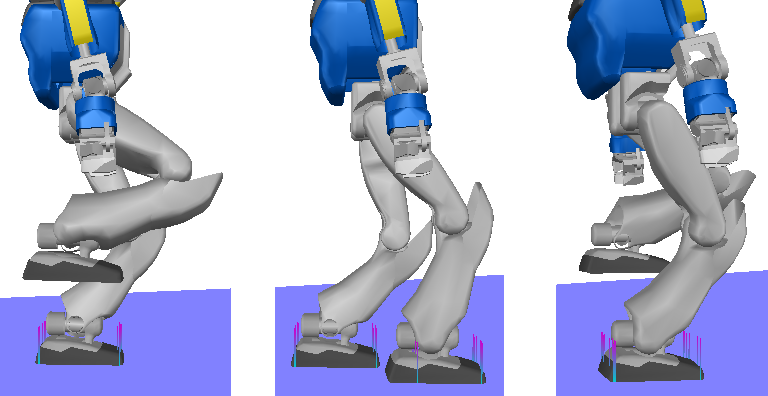
\includegraphics[width=8cm]{./images/HalfStep.png}\\
    \end{figure}
   \end{center}
  Un pas complet se fait en 4 phases :
  \begin{small}
    \begin{itemize}
    \item Phase stable de simple support
    \item Phase de vol
    \item Phase stable de double support
    \item Phase de vol
    %\item Phase stable de simple support
    \end{itemize}
    \end{small}
\end{frame}

\section{Volumes balayés}
\begin{frame}
  \center Approximation des volumes balayés
  \begin{tiny}
    \begin{figure}
      \subfigure[\tiny{Original - 1.687.596}]{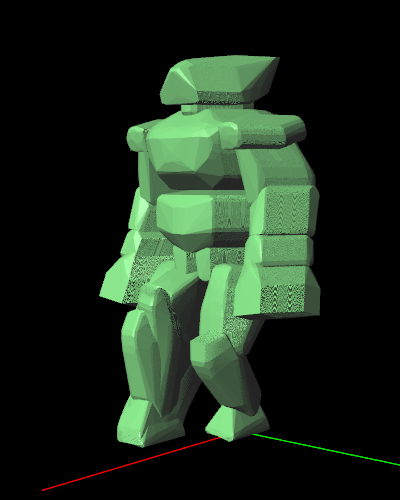
\includegraphics[width=2.5cm]{./images/SV_original.png}}~
      \subfigure[\tiny{5mm - 508.120}]{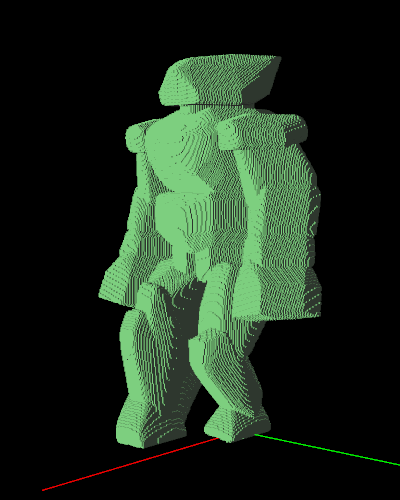
\includegraphics[width=2.5cm]{./images/SV_5mm.png}}~
      \subfigure[\tiny{10mm - 125.772}]{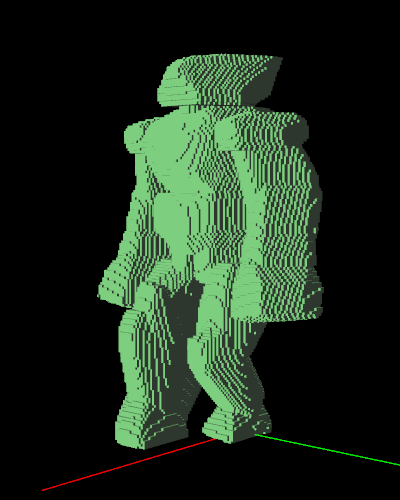
\includegraphics[width=2.5cm]{./images/SV_10mm.png}}
    \end{figure}
    \vspace{-7mm}
    \begin{figure}
      \subfigure[\tiny{25mm - 19.524}]{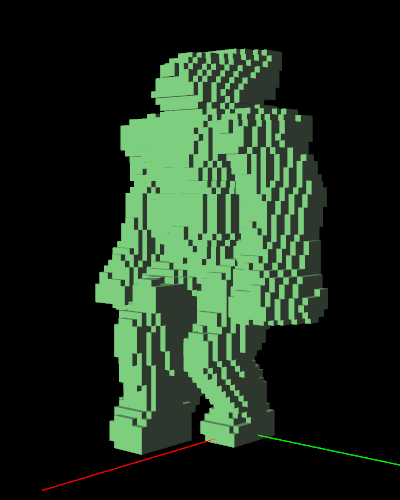
\includegraphics[width=2.5cm]{./images/SV_25mm.png}}~
      \subfigure[\tiny{50mm - 4.596}]{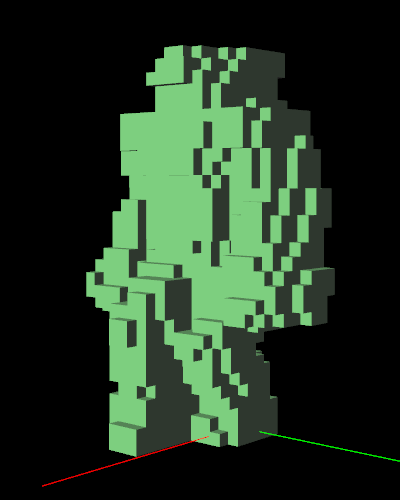
\includegraphics[width=2.5cm]{./images/SV_50mm.png}}~
      \subfigure[\tiny{100mm - 1.144}]{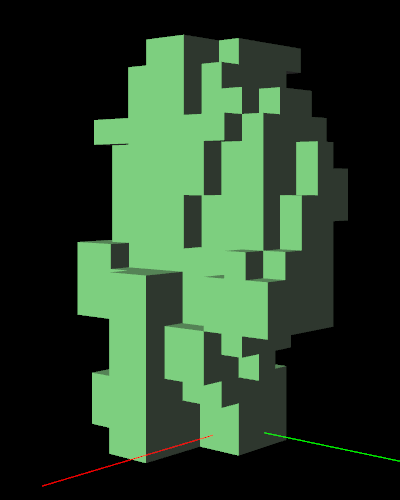
\includegraphics[width=2.5cm]{./images/SV_100mm.png}}
    \end{figure}
  \end{tiny}
\end{frame}

\section{Lissage de trajectoire}
\begin{frame}
  \begin{center} 
    Accélération des trajectoires
    \begin{figure}
      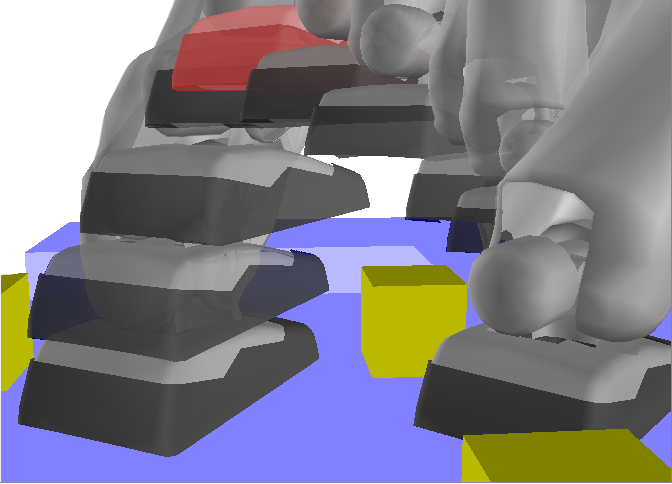
\includegraphics[width=5cm]{./images/smoothing_before.png}~
      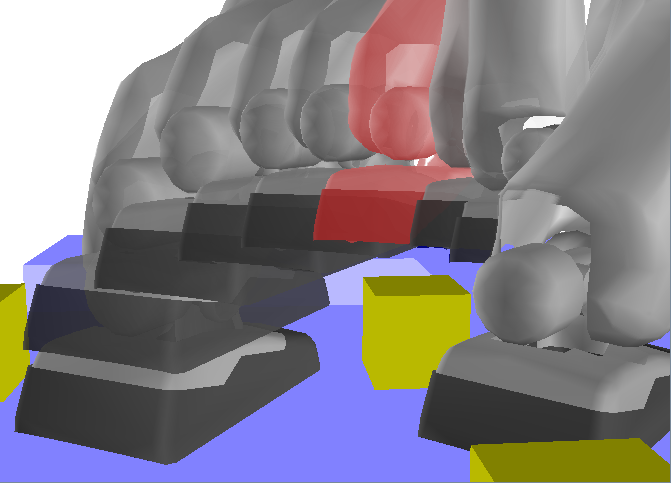
\includegraphics[width=5cm]{./images/smoothing_after.png}
    \end{figure}
    
    Suppression de la phase de double support\\
    Réduction au mieux de la phase de simple support
  \end{center}
\end{frame}

\section{Matériel}
\begin{frame}
  \begin{figure}
    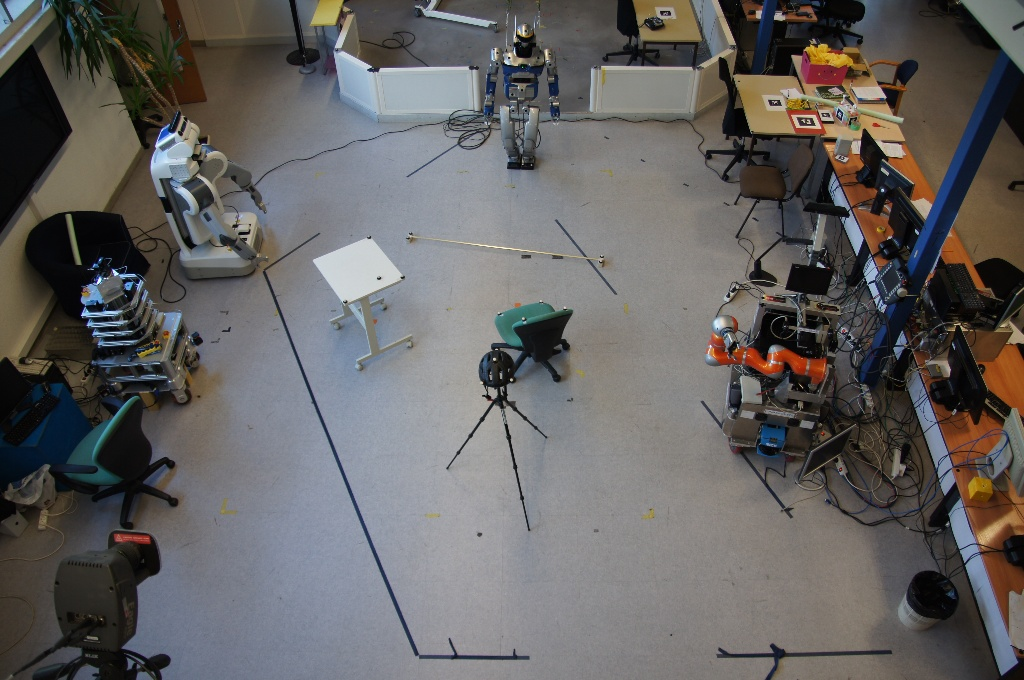
\includegraphics[width=9cm]{./images/grande_salle.jpg}\\
    Grande salle d'expérience robotique du LAAS.
  \end{figure}
\end{frame}

\section{Motion capture}
\begin{frame}
  \center Détection des différents objets avec la \textit{motion capture}.\\
   \begin{figure}
    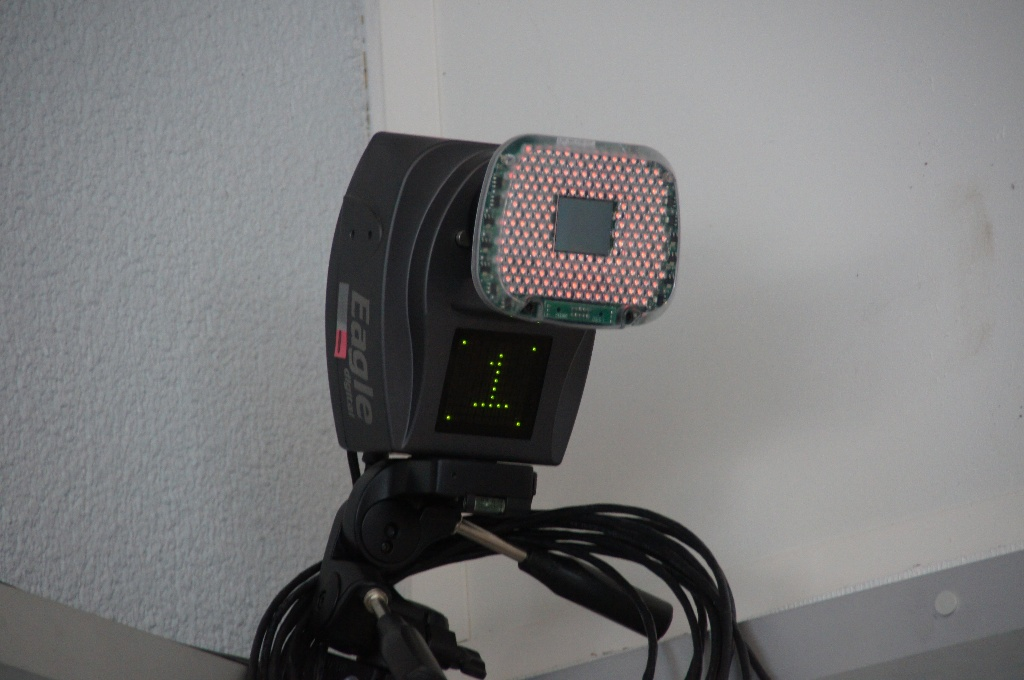
\includegraphics[width=4.5cm]{./images/IR.jpg}~
    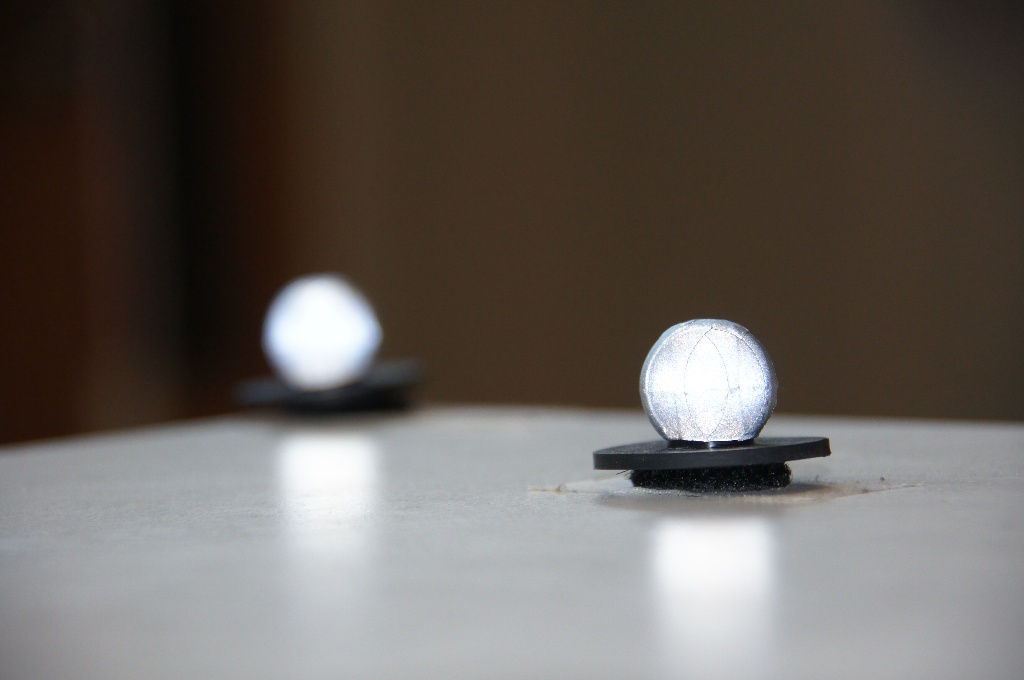
\includegraphics[width=4.5cm]{./images/marker_flash.jpg}
  \end{figure}
  \vspace{-5mm}
  \begin{figure}
    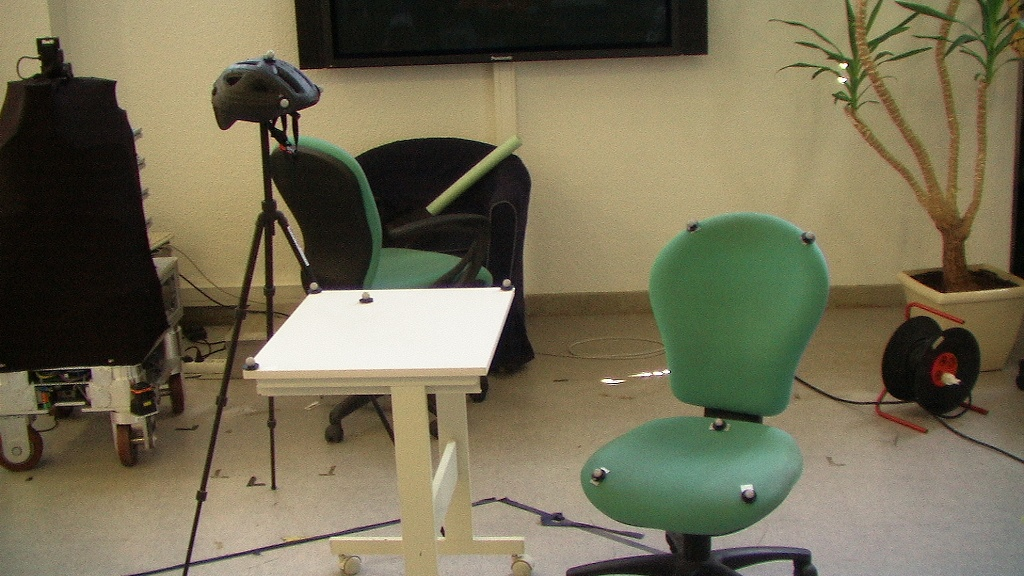
\includegraphics[width=5cm]{./images/mocap_real.jpg}~
    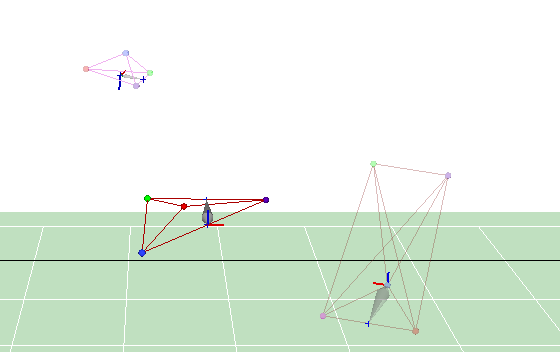
\includegraphics[width=5cm]{./images/mocap.png}
  \end{figure}
\end{frame}

\end{document}